\section*{Exercice 154 -- Treuil de levage}


\textit{D'après ressources Pole Chateaubriand -- Joliot-Curie.}
\setcounter{exo}{0}
\ifprof
\else
On s’intéresse à un treuil dont la photo et le modèle cinématique sont donnés ci-dessous.
\begin{center}
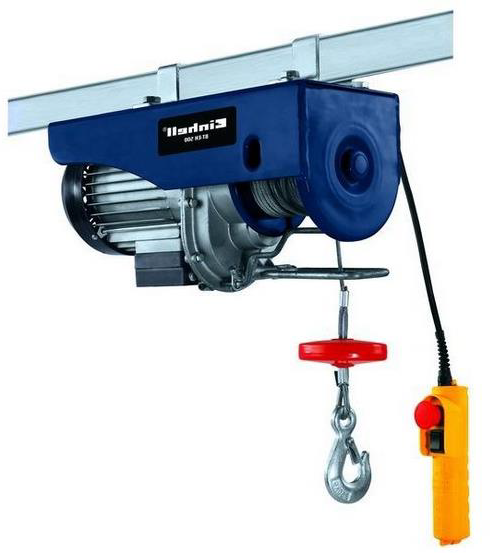
\includegraphics[width=.5\linewidth]{063_01}
\end{center}

\begin{center}
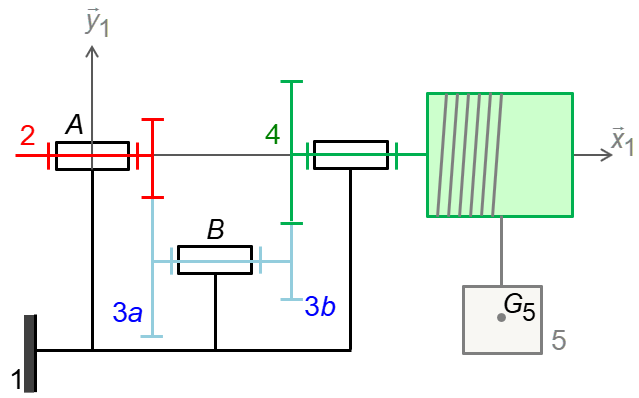
\includegraphics[width=\linewidth]{063_02}
\end{center}

On note $Z_2$ le nombre de dents de la roue dentée de l'arbre 2. On note l'arbre intermédiaire 3 et $Z_{3a}$ et $Z_{3b}$ les nombres de dents de ses deux roues dentées. On note $R$ le rayon du tambour 4 sur lequel s’enroule sans glisser un câble et $Z_4$ le nombre de dents de sa roue dentée.

\fi

\subparagraph{}
\textit{Déterminer la relation entre $v_{51}$ la vitesse de déplacement de la charge par rapport au bâti et $\omega_{21}$ la vitesse de rotation du moteur.}
\ifprof
\begin{corrige}
\end{corrige}
\else
\fi


\subparagraph{}
\textit{On note $J_2$, $J_3$, $J_4$ l'inertie des pièces 2, 3 et 5. On note $M_5$ la masse du solide 5. Donner la masse équivalente ramenée << à la translation >> de la masse. Donner l'inertie équivalente ramenée à l'arbre d'entrée 2.  }
\ifprof
\begin{corrige}
\end{corrige}
\else
\fi
